\section{Statistical Models}
\label{ch:statmodel}

Primary source for this was Hyndman-et-al-2018 \cite{Hyndman-et-al-2018}.

Some of our statistical models require \textit{homoscedasticity}, i.e., that the model errors are identically distributed with the same variance $\sigma^2$.

We can check this by plotting standardized residuals and checking that they are distributed around zero, with 95 percent of the values within the interval $[1.96,1.96]$

\begin{figure}[h]
\minipage{0.33\textwidth}
  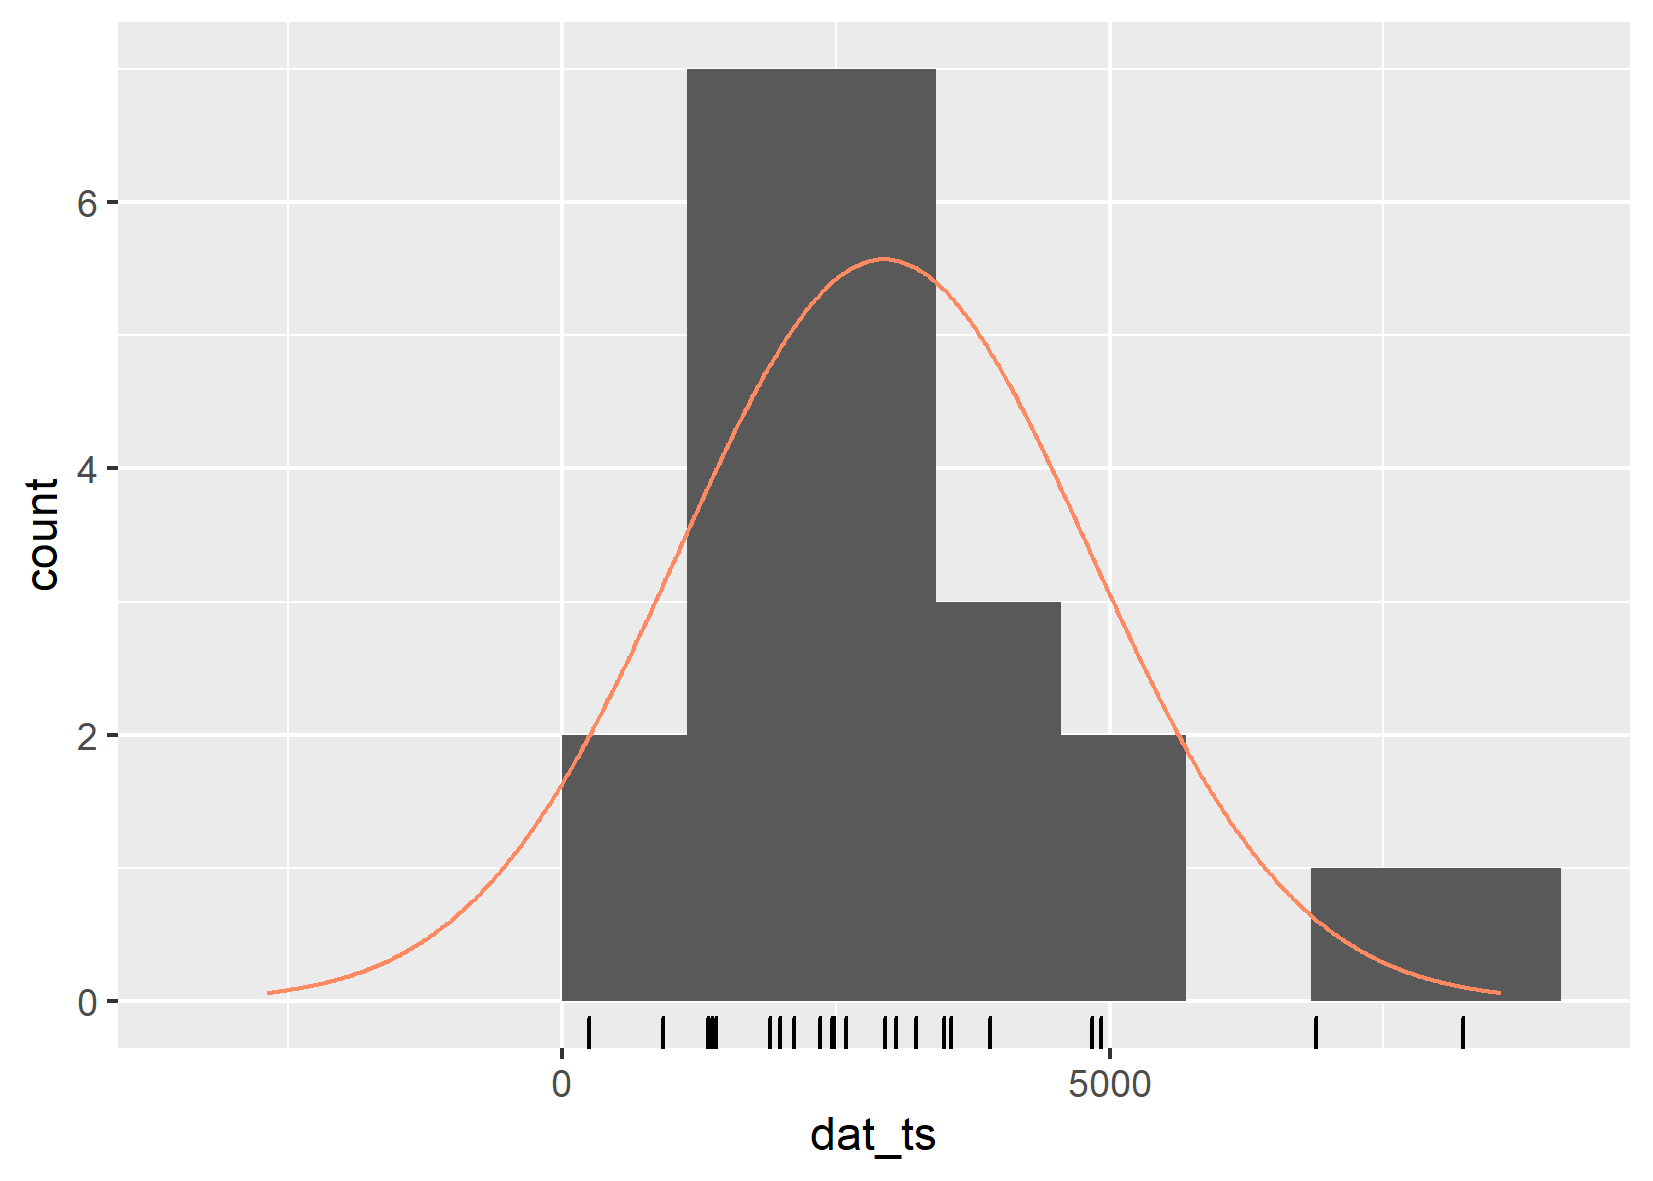
\includegraphics[width=\linewidth]{Ireland-residuals.png} \label{fig:ireland-residuals}
\endminipage\hfill
\minipage{0.33\textwidth}
  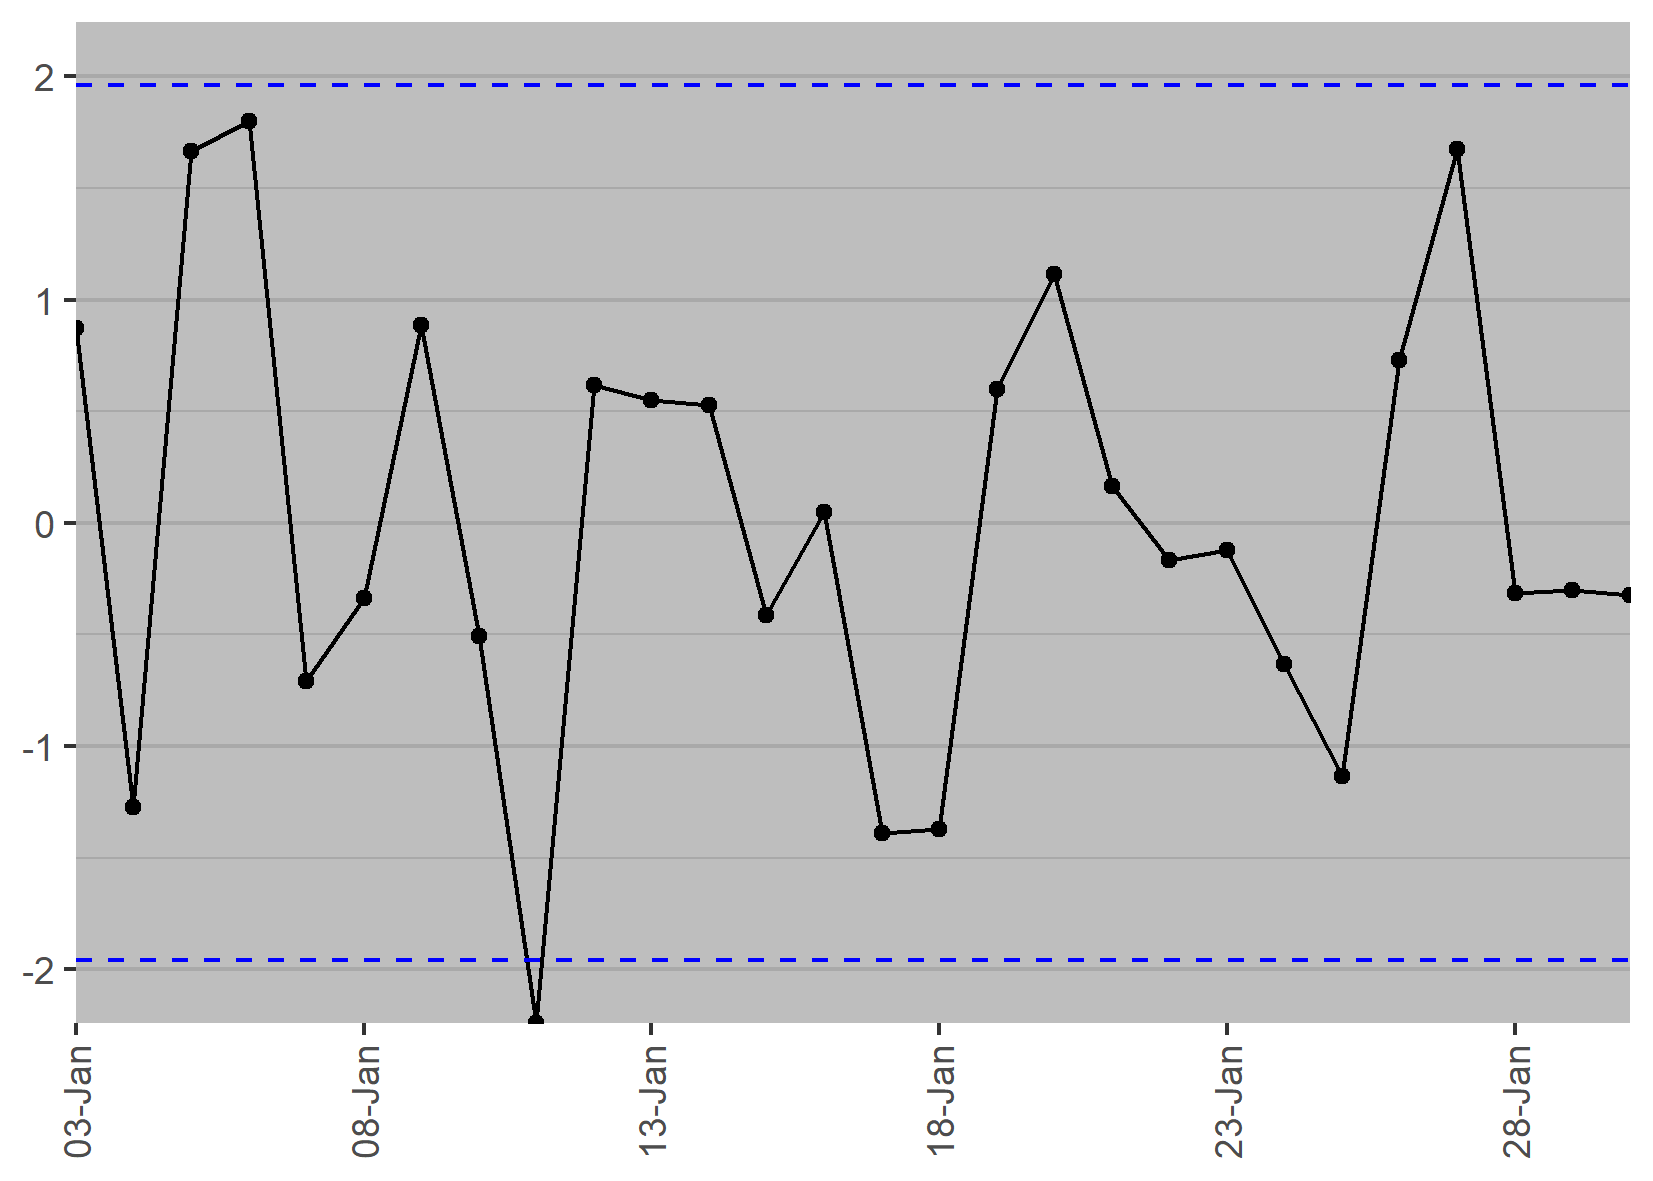
\includegraphics[width=\linewidth]{Italy-residuals.png} \label{fig:italy-residuals}
\endminipage\hfill
\minipage{0.33\textwidth}
  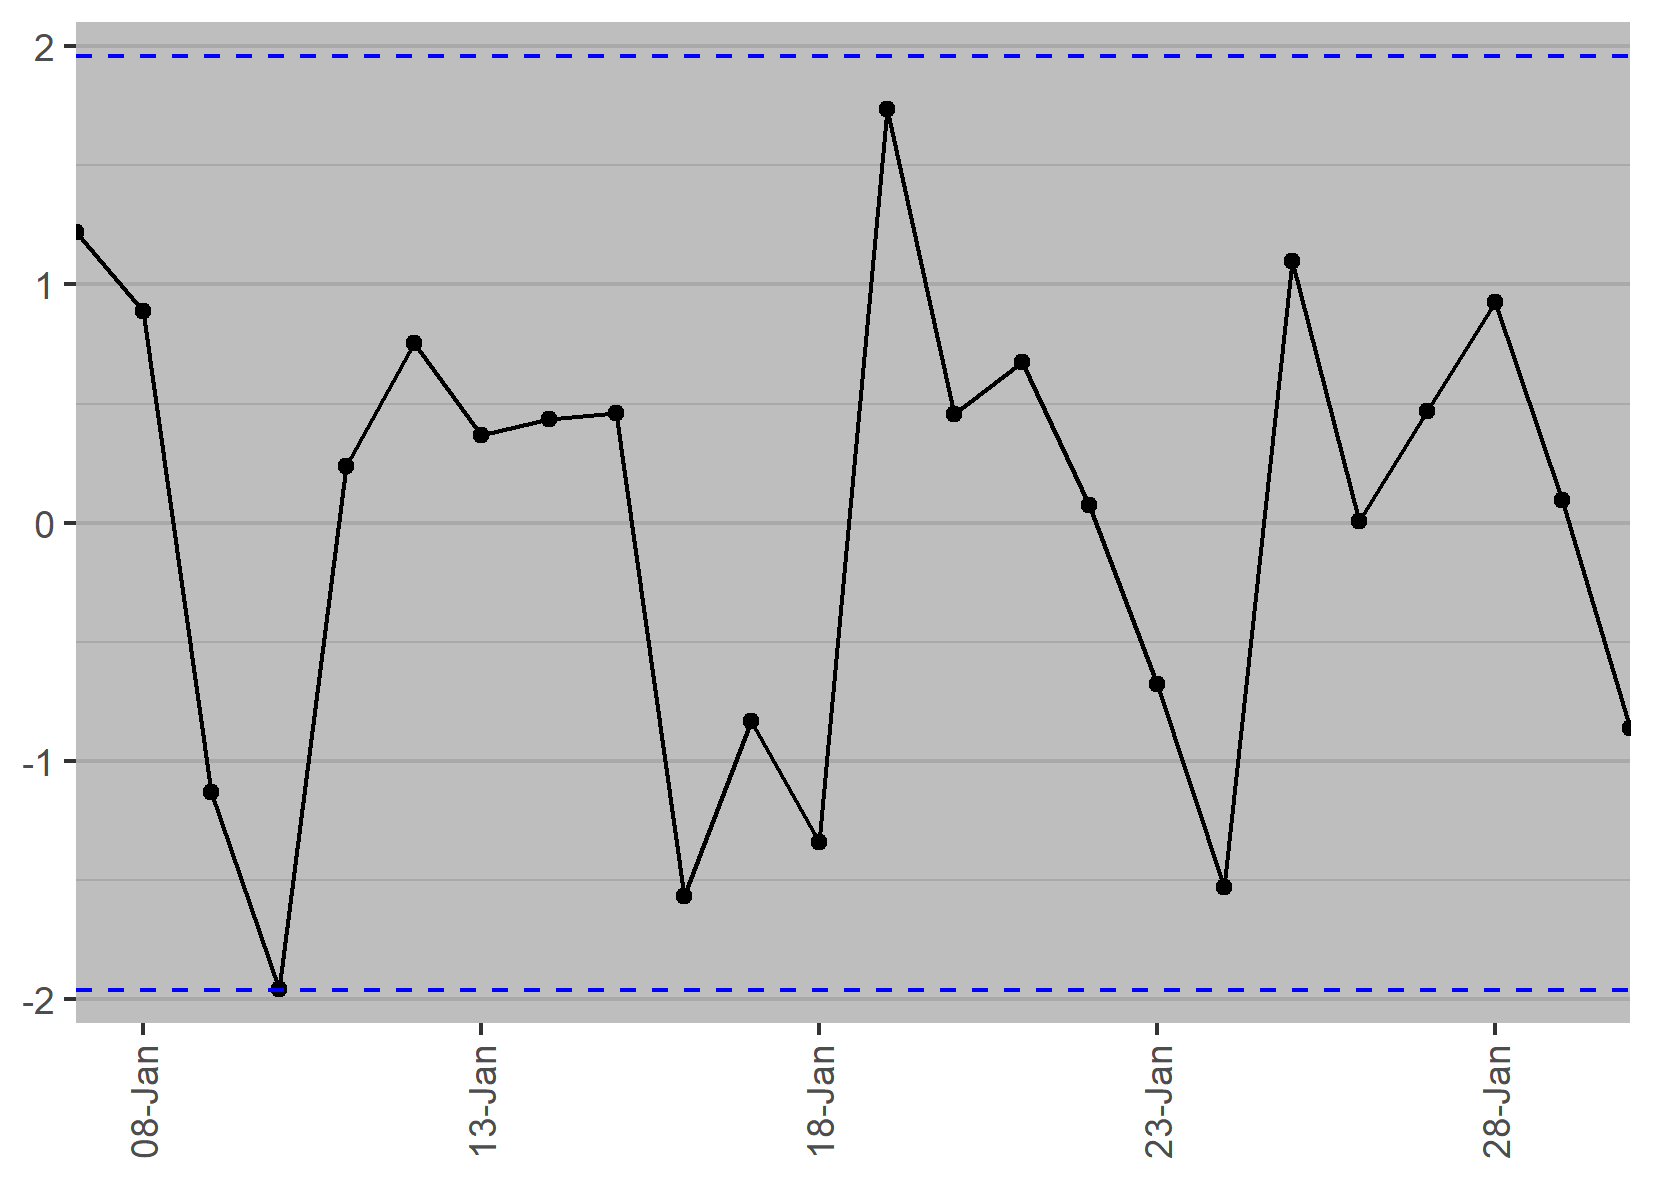
\includegraphics[width=\linewidth]{United States-residuals.png} \label{fig:usa-residuals}
\endminipage\hfill
\caption{Residual checks, Ireland, Italy and United States}
\end{figure}

\subsection{Holt-Winters’ seasonal method}

\subsubsection{Definitions and Theory}

\begin{figure}
\begin{tcolorbox}[width=.6\textwidth]%

Suppose there are $N$ observations.

Initial step:

$\left|\begin{array}{l}
L_s = \frac1s \sum_{i=1}^s y_i \\
b_s = \frac1s \left[\frac{y_{s+1}-y_1}{s}+\frac{y_{s+2}-y_2}{s}+\dots+\frac{y_{2s}-y_s}{s}\right]\\
S_i  = y_i-L_s, \ i=1,\dots,s
\end{array}\right.$

and choose parameters $0\leq\alpha\leq1,\ 0\leq\beta\leq1$ and $0\leq\gamma\leq1$

Then compute for $s<t\leq N$:

$\left|\begin{array}{lll}
\text{Level} &       L_t & = \alpha (y_t-S_{t-s})+(1-\alpha)(L_{t-1}+b_{t-1})\\
\text{Trend} &      b_t & = \beta(L_t-L_{t-1})+(1-\beta)b_{t-1}\\
\text{Seasonal} & S_t & = \gamma (y_t-L_t) + (1-\gamma)S_{t-s}\\
\text{Forecast} & F_{t+1} & = T_t+b_t+S_{t+1-s}
\end{array}\right.$
For subsequent observations,

$F_{N+k}=L_N+k\cdot b_N+S_{N+k-s}$
\label{SHWx}
\end{tcolorbox}
\caption{Seasonal Holt Winter’s Multiplicative Model Algorithm (denoted SHW$_{+}$)}
\end{figure}


\subsubsection{How to select the best model}

\subsubsection{Forecasting}

\subsubsection{implementation in R}


We see that the additive seasonal method is a better choice for both model fit and confidence interval size.

\begin{figure}[h]
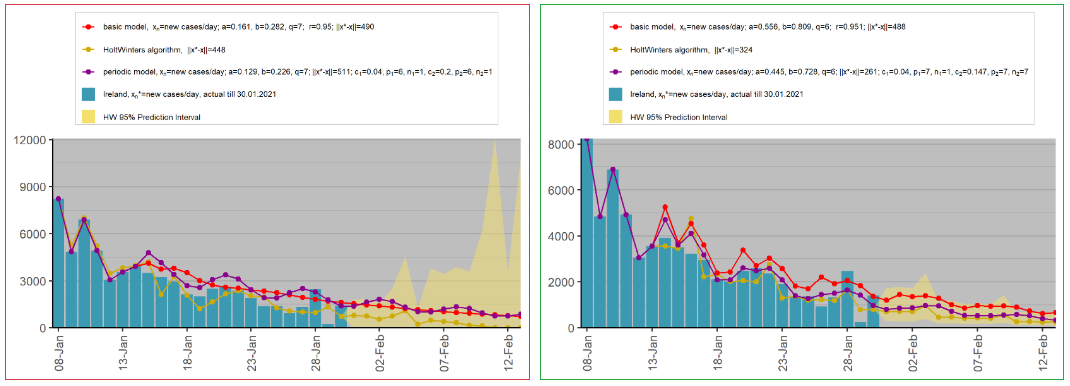
\includegraphics[width=0.9\textwidth]{hwaddmultcompare.png}
\caption{Comparison between HoltWinters multiplicative (left, red outline) and additive (right, green outline)algorithms, at some point during the research}
\end{figure}

\begin{figure}[!htb]
\minipage{0.48\textwidth}
  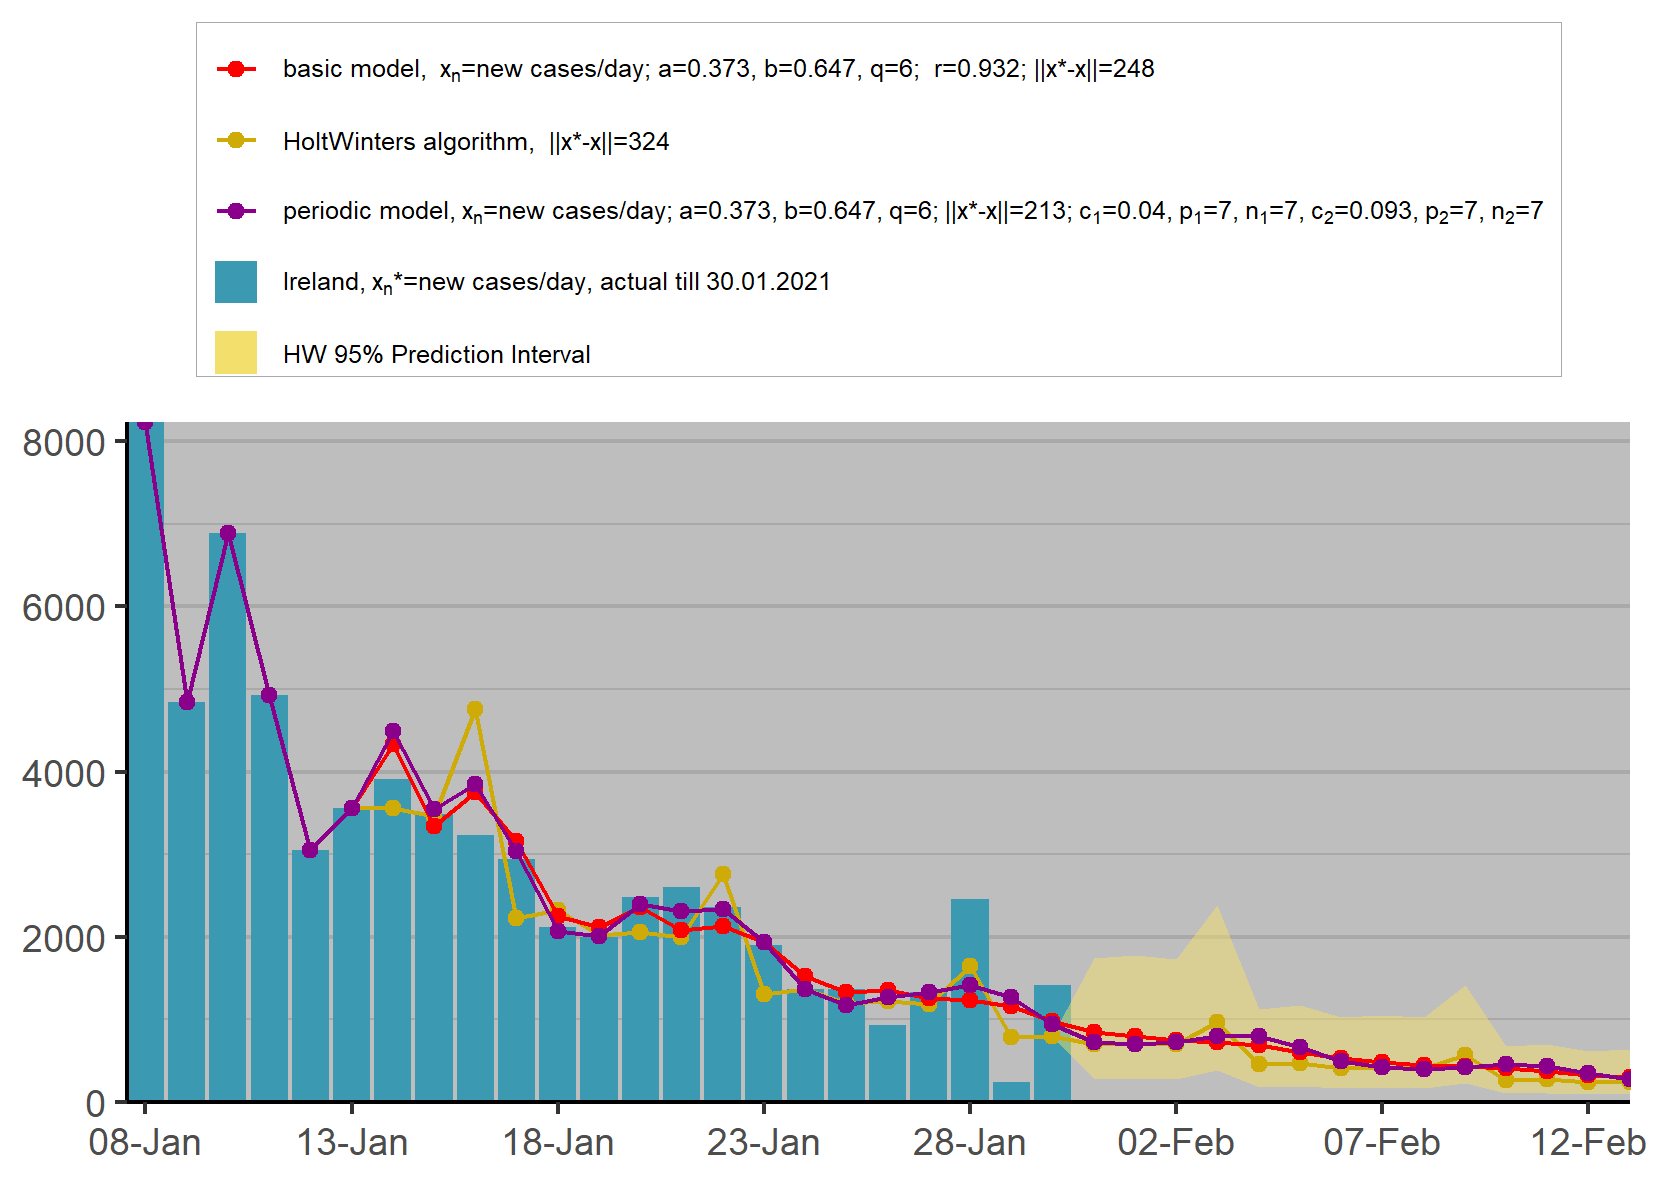
\includegraphics[width=\linewidth]{Ireland-hw.png} \label{fig:ireland-hw}
\endminipage\hfill
\minipage{0.48\textwidth}
  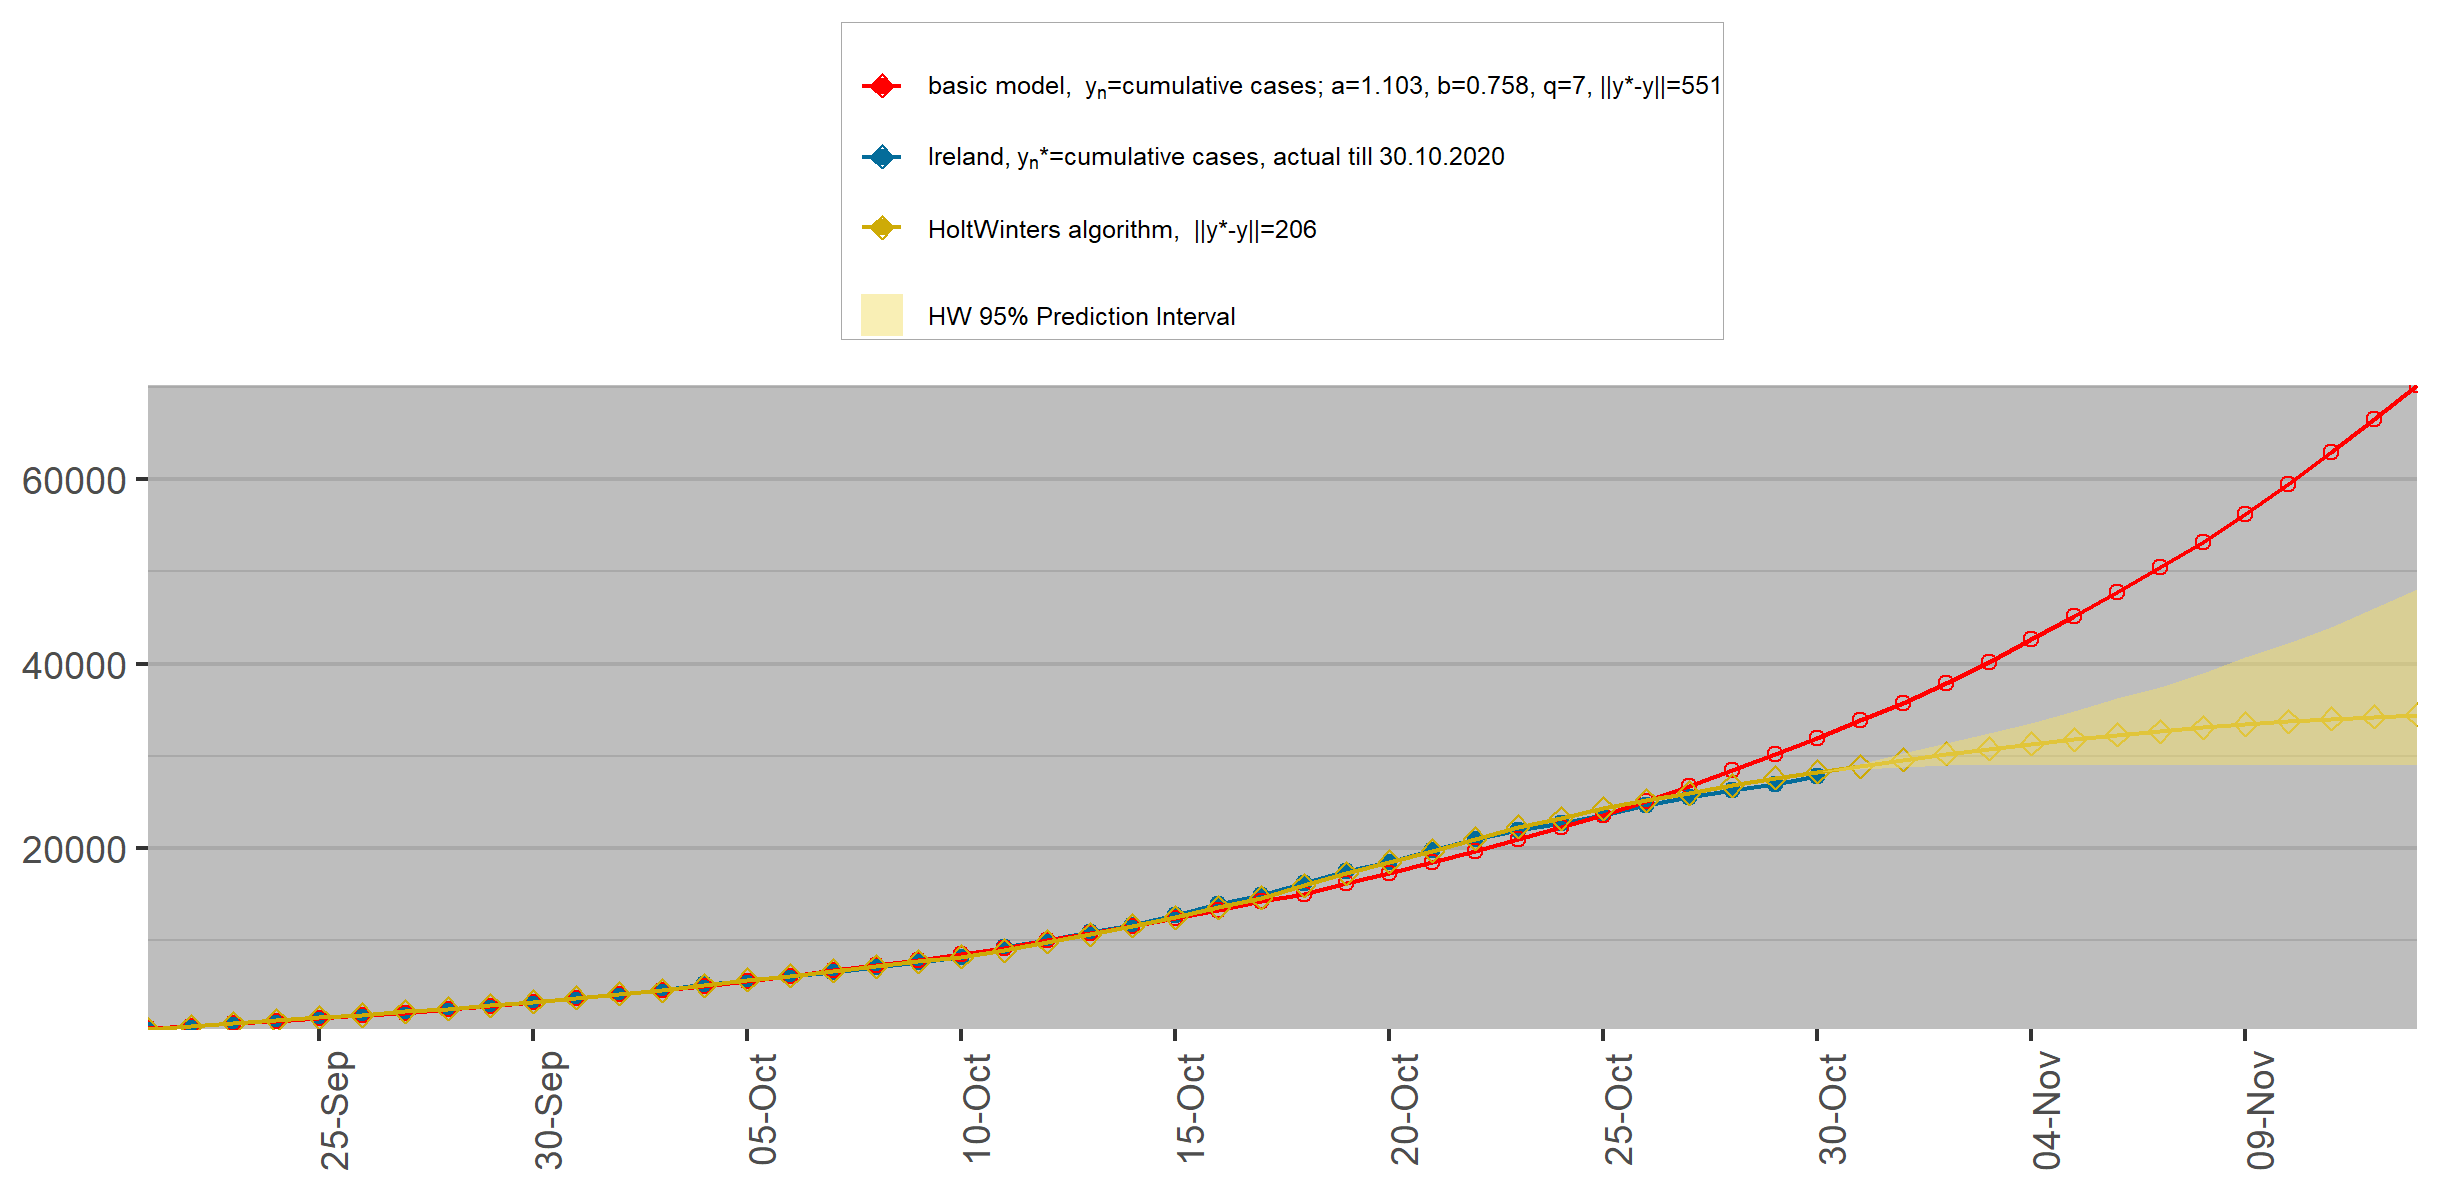
\includegraphics[width=\linewidth]{Ireland-hwy.png} \label{fig:ireland-hwy}
\endminipage
\caption{HoldWinters model, Ireland}
\end{figure}


\subsection{ARIMA models}

\begin{definition}
The \textit{backshift operator} $B$ is a function on a time series $\left(x_n\right)_{n\geq1}$ such that $Bx_n=x_{n-1}$ and more genrerally:

$$B^k x_n= x_{n-k},\quad n>k$$

And similarly for the independent errors $\eps_n$:

$$B^k \eps_n= \eps_{n-k},\quad n>k$$
\end{definition}

We must first define the each component of a non-seasonal ARIMA model (suitable for time series with a trend).

\begin{itemize}
\item An $AR(p)$ model, or an autoregressive model of order $p$ of a time series $x_1,\dots,x_N$ states that each $x_n$ is a \textit{linear function} of $x_{n-p},x_{n-p+1},\dots,x_{n-1}$ and an error term, i.e. 
$$x_n= \phi_0+\phi_1 x_{n-1}+\phi_2 x_{n-2} +\dots + \phi_p x_{n-p}+\eps_n,\quad n>p,\quad \eps_n\sim N(0,\sigma^2)$$

We can simplify using the backshift operator $B$:

\begin{align}
x_n
&= \phi_0+\phi_1 Bx_n+\phi_2 B^2x_n +\dots + \phi_p B^px_n +\eps_n\nonumber \\
&= \phi_0+\left(\phi_1 B+\phi_2 B^2 +\dots + \phi_p B^p\right)x_n +\eps_n
\end{align}

\item An $MA(q)$ model, or a moving average model of order $q$ of a time series $x_1,\dots,x_N$ states that each $x_n$ is a \textit{linear function} of the $q$ previous errors $\eps_{n-q},\eps_{n-q+1},\dots,\eps_{n-1}$, plus the current error $\eps_n$, i.e. 
$$x_n= \psi_0-\psi_1 \eps_{n-1}-\psi_2 \eps_{n-2} -\dots - \psi_q \eps_{n-p}+\eps_n,\quad n>p$$

By convention we use minus signs in the coefficients $\psi_1,\dots,\psi_q$
We can simplify using the backshift operator $B$:

\begin{align}
x_n
&= \psi_0-\psi_1 B\eps_n-\psi_2 B^2\eps_n -\dots - \psi_q B^q\eps_n + \eps_n \nonumber \\
&= \psi_0+\left(1-\psi_1 B-\psi_2 B^2 +\dots - \psi_q B^q\right)\eps_n 
\end{align}

\item The first order differencing of the time series, $I(1)$, is evalueated as 

\begin{align}
x_n'
&=x_n-x_{n-1}\nonumber \\
&=x_n-Bx_n \nonumber \\
&=\left(1-B\right)x_n
\end{align}

More generally, the differencing of order $d$, denoted $I(d)$ is 
$$(1-B)^d x_n$$

This only affects the $y_n$ (although constants are differenced to zero) and the errors $\eps_n$ are unchanged.
\end{itemize}

Therefore, an ARIMA$(p,d,q)$ model can be evaluated by combining the $AR(p),\ I(d)$ and $MA(q)$

\begin{align}
(1-B)^d x_n
&= \phi_0+(1-B)^d\left(\phi_1 B+\phi_2 B^2 +\dots + \phi_p B^p\right)x_n +
\psi_0+\left(\psi_1 B+\psi_2 B^2 +\dots + \psi_q B^q\right)\eps_n \nonumber 
\end{align}

\begin{align}
(1-B)^d x_n + (1-B)^d\left(-\phi_1 B-\phi_2 B^2 -\dots - \phi_p B^p\right)x_n
&= \phi_0 + \psi_0+\left(1-\psi_1 B-\psi_2 B^2 +\dots - \psi_q B^q\right)\eps_n  \nonumber \\
(1-B)^d\left(1-\phi_1 B-\phi_2 B^2 -\dots - \phi_p B^p\right)x_n
&=c+\left(1-\psi_1 B-\psi_2 B^2 +\dots - \psi_q B^q\right)\eps_n  \nonumber \\
\end{align}

where $c= \phi_0 + \psi_0$ (it is zero if $d\geq1$.

We also need the seasonal components for an ARIMA$(p,d,q)(P,D,Q)_s$ 

Suppose a time series $x_n$ has period $s$ (seasonal pattern every $s$ values)
\begin{itemize}

\item An $AR(P)_s$ model, or a seasonal autoregressive model of order $P$ of a time series $x_1,\dots,x_N$ states that each $x_n$ is a \textit{linear function} of $x_{n-Ps},x_{n-(P-1)s},\dots,x_{n-s}$ and an error term, i.e. 
$$x_n= \beta_0+\beta_1 x_{n-s}+\beta_2 x_{n-2s} +\dots + \beta_P x_{n-Ps}+\eps_n$$

We can simplify using the backshift operator $B$:

\begin{align}
x_n &= \beta_0+\left(\beta_1 B^s+\beta_2 B^{2s} +\dots + \beta_P B^{Ps}\right)x_n
\end{align}

\item An $MA(Q)_s$ model, or a seasonal moving average model of order $Q$ of a time series $x_1,\dots,x_N$ states that each $x_n$ is a \textit{linear function} of the $Q$ errors $\eps_{n-Ws},\eps_{n-(Q-1)s},\dots,\eps_{n-s}$, plus the current error $\eps_n$, i.e. 
$$x_n= \gamma_0-\gamma_1 \eps_{n-s}-\gamma_2 \eps_{n-2s} -\dots - \gamma_Q \eps_{n-Qs}+\eps_n$$

Again, by convention we use minus signs in the coefficients $\gamma_1,\dots,\gamma_Q$

We can simplify using the backshift operator $B$:

\begin{align}
x_n
&= \gamma_0-\gamma_1 \eps_{n-s}-\gamma_2 \eps_{n-2s} -\dots - \gamma_Q \eps_{n-Qs}+\eps_n \nonumber \\
&= \gamma_0+\left(1-\gamma_1 B^s-\gamma_2 B^{2s} +\dots - \gamma_Q B^{Qs}\right)\eps_n 
\end{align}

\item The first order seasonal differencing of the time series, $I_s(1)$, is evalueated as 

$$x_n-x_{n-s}=\left(1-B^s\right)x_n$$

More generally, the seasonal differencing of order $D$, denoted $I_s(D)$ is 

$$(1-B^s)^D x_n$$

The purpose of this is to make the time series  stationary in mean
\end{itemize}


Then we can similarly compose our seasonal components with the previous ARIMA$(pd,q)$ to get the definition of an ARIMA$(p,d,q)(P,D,Q)_s$ model

\begin{align}
\underbrace{\left(1-\phi_1 B-\phi_2B^2-\dots-\phi_p B^p\right)}_{AR(p)}
\underbrace{\left(1-\beta_1 B^s-\beta_2B^{2s}-\dots-\beta_P B^{Ps}\right)}_{AR_s(P)} 
\underbrace{\left(1-B\right)^d}_{I(d)}\underbrace{\left(1-B^s\right)^D}_{I_s(D)}   y_n = \nonumber \\
 c+
\underbrace{\left(1-\psi_1 B-\psi_2B^2-\dots-\psi_q B^q\right)}_{MA(q)}
\underbrace{\left(1-\gamma_1 B^s-\gamma_2B^{2s}-\dots-\gamma_Q B^{Qs}\right)}_{MA_s(Q)} \eps_n
\end{align}

where the constant $c$ is some function of the constants $\phi_0,\psi_0,\beta_0$ and $\gamma_0$ 

\subsubsection{How to select the best model}

\subsection{Forecasting}

\subsubsection{implementation in R}


\begin{figure}[h]
\minipage{0.48\textwidth}
  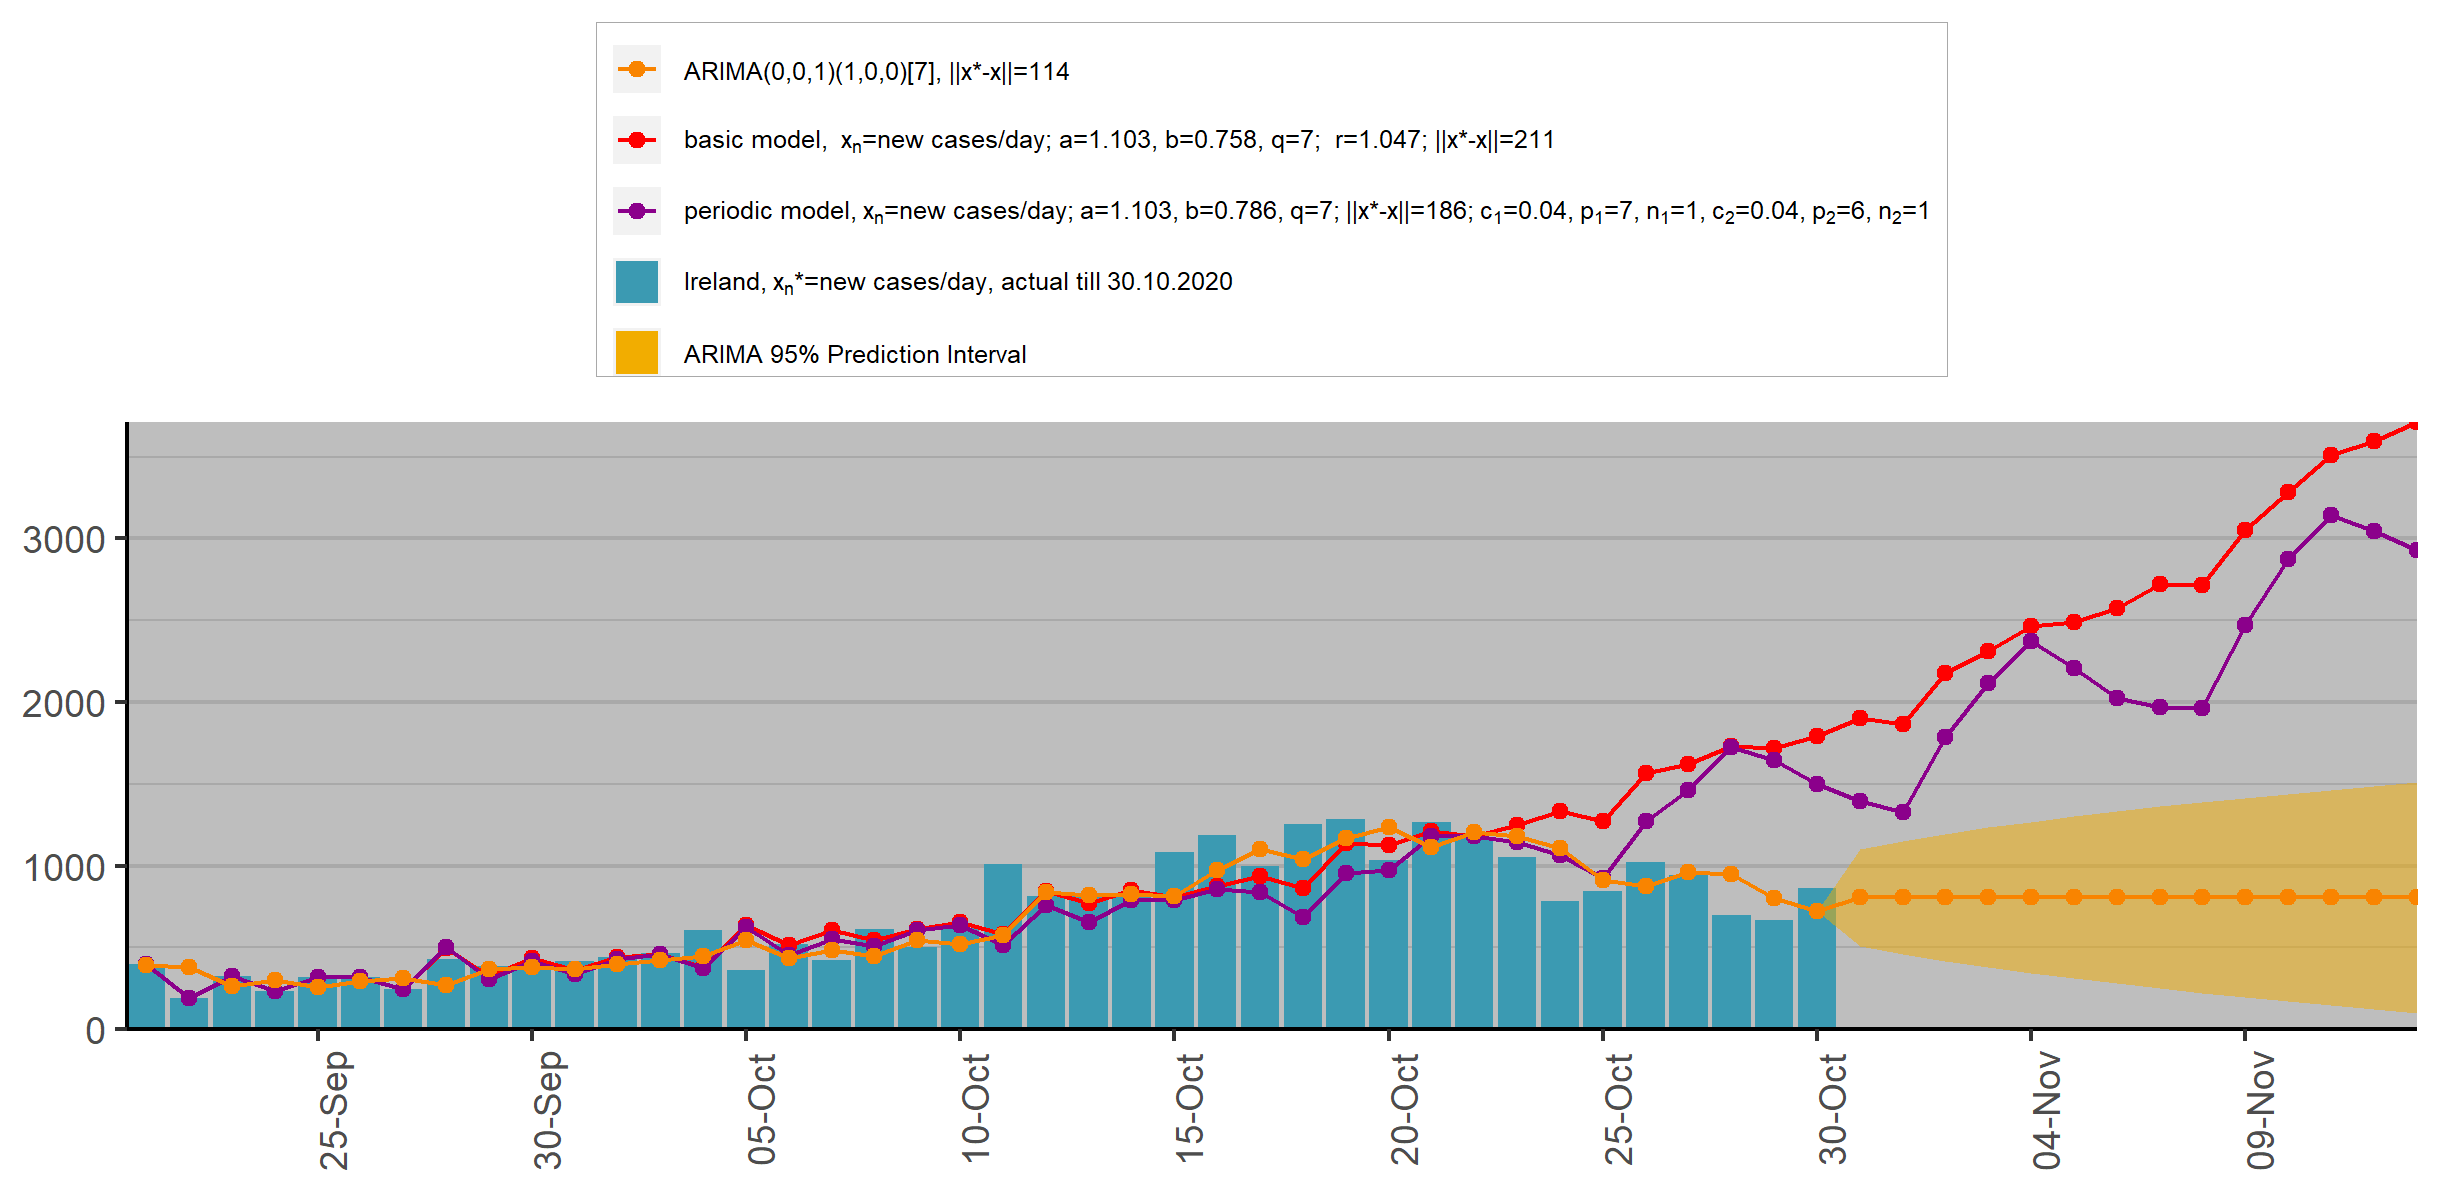
\includegraphics[width=\linewidth]{Ireland-arima.png} \label{fig:ireland-arima}
\endminipage\hfill
\minipage{0.48\textwidth}
  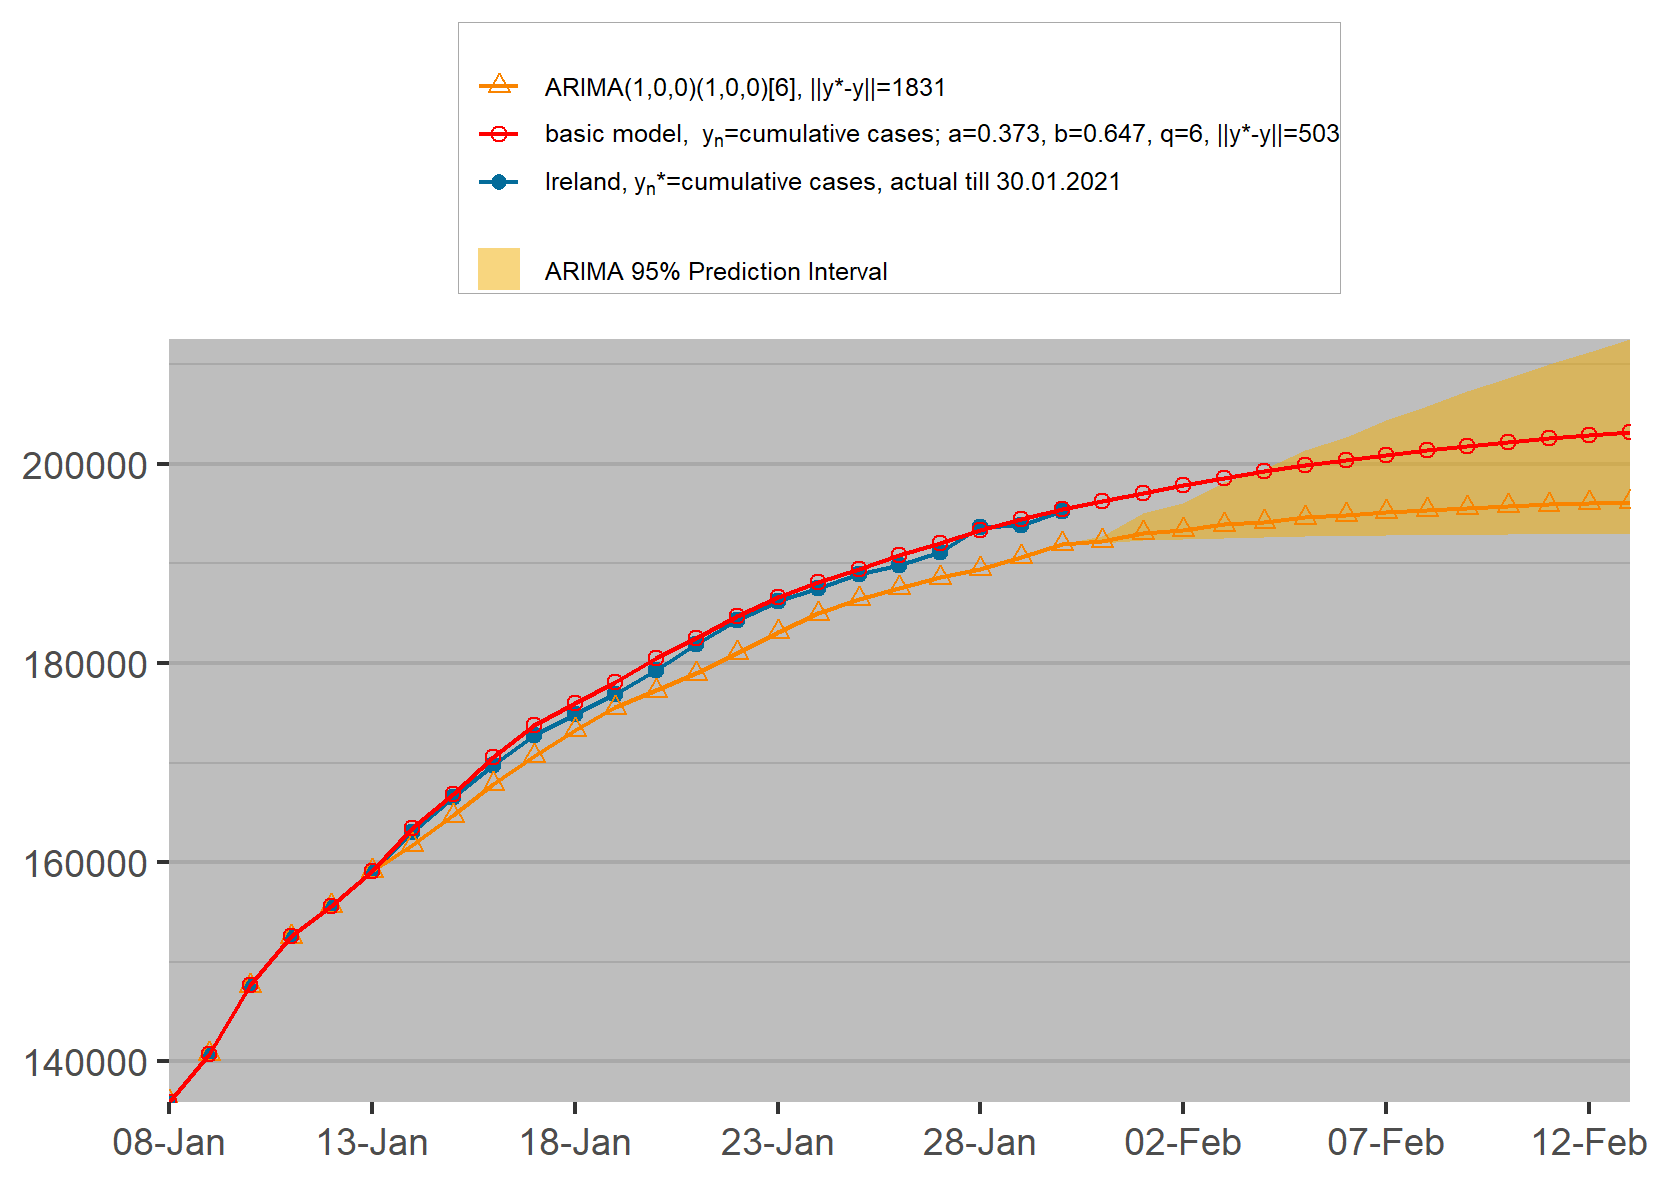
\includegraphics[width=\linewidth]{Ireland-arimay.png} \label{fig:ireland-arimay}
\endminipage
\caption{ARIMA model, Ireland}
\end{figure}

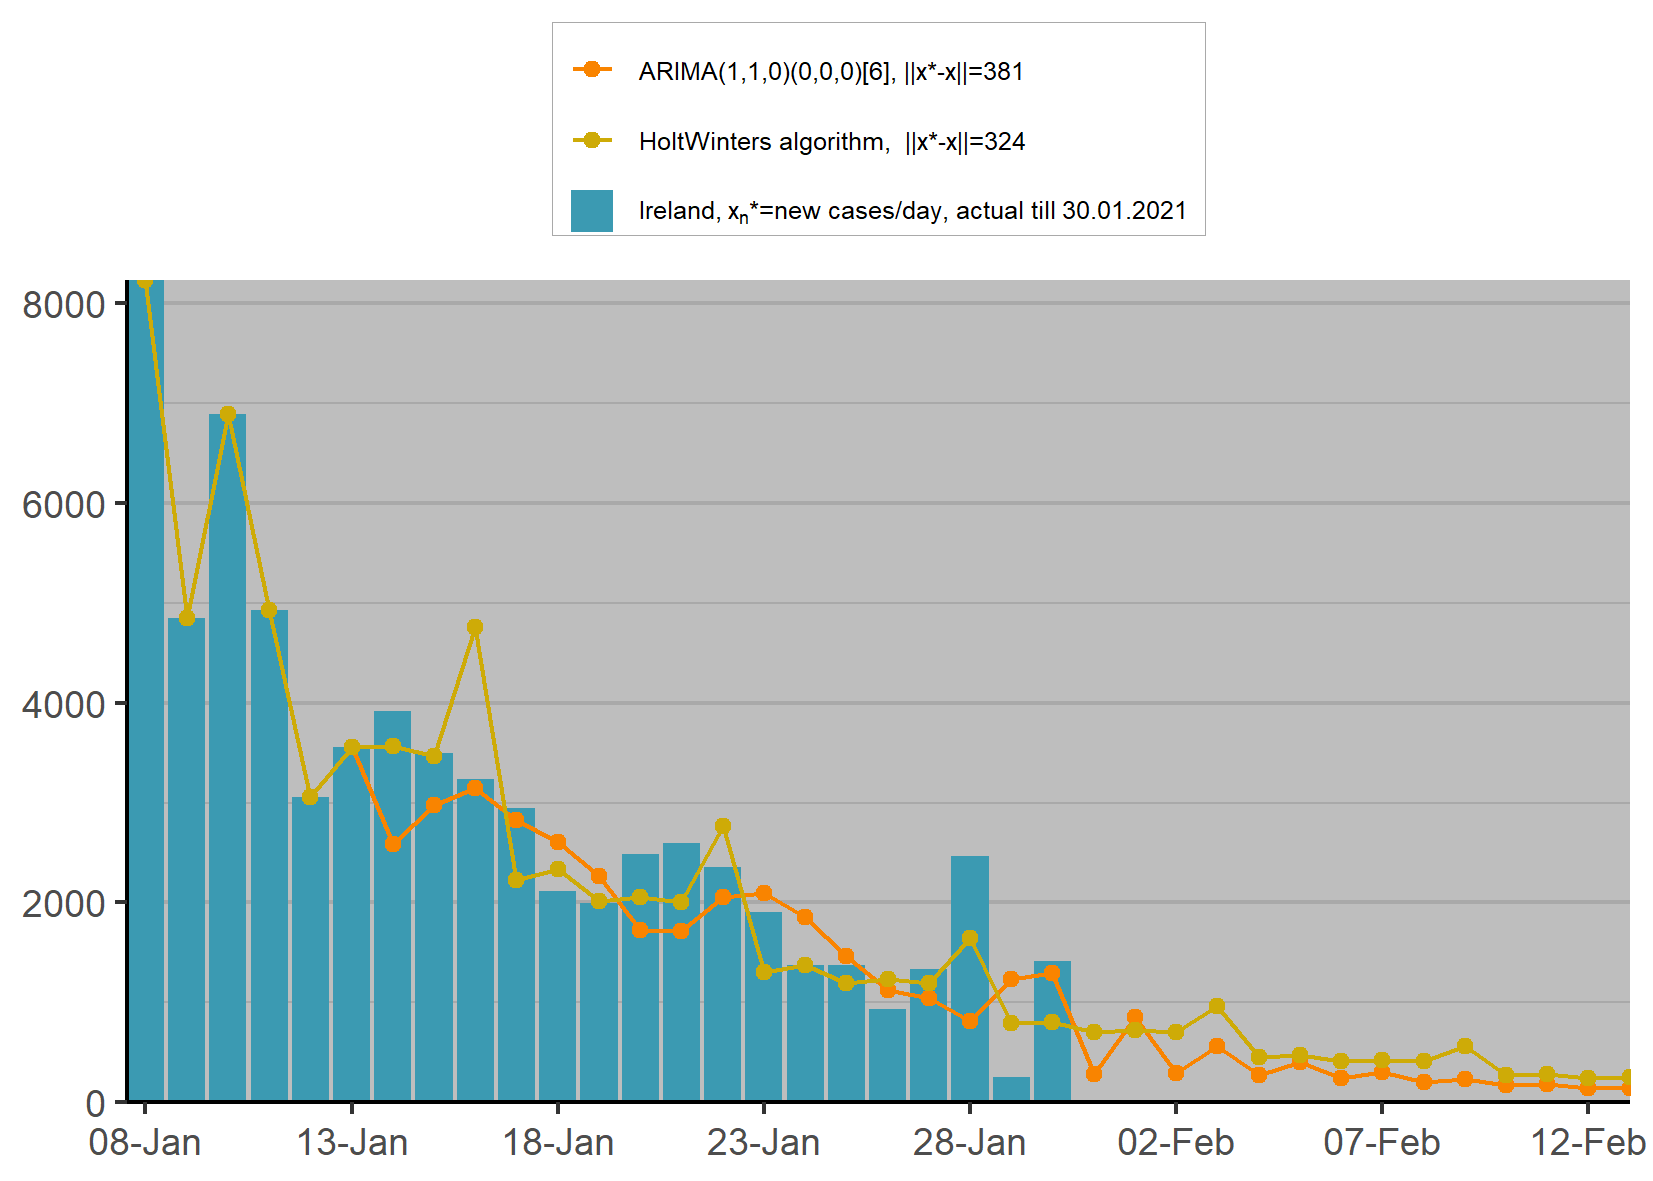
\includegraphics[width=0.9\textwidth]{Ireland-hwarima.png}


\subsection{Neural network models}

\subsubsection{Definitions and Theory}

\subsubsection{How to select the best model}

\subsubsection{Forecasting}

\subsubsection{implementation in R}

\begin{figure}[h]
\minipage{0.48\textwidth}
  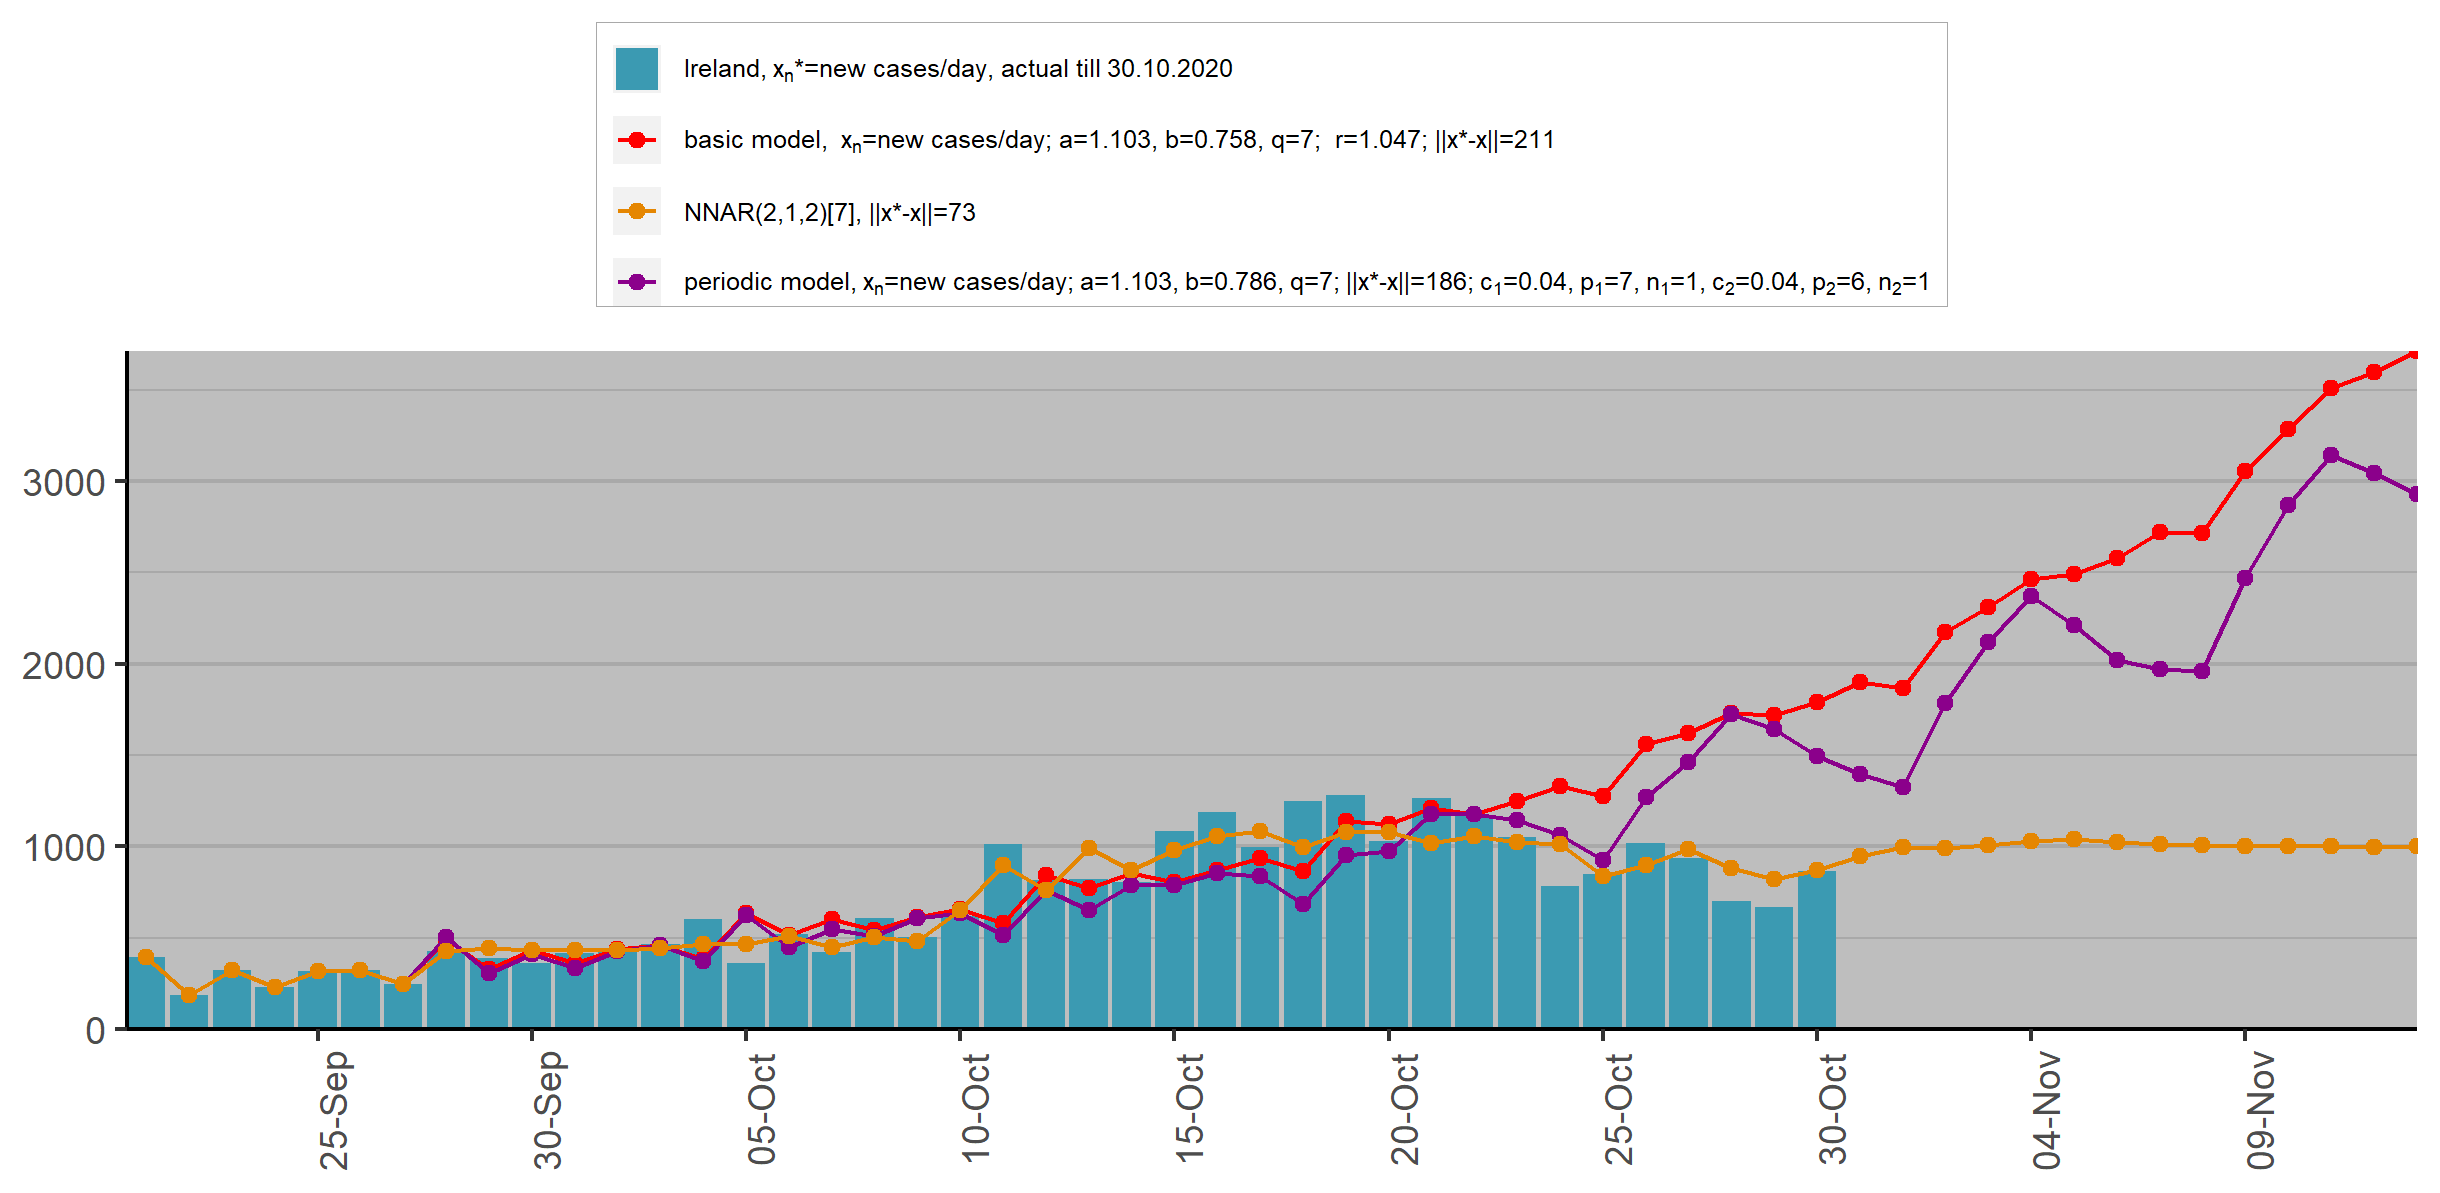
\includegraphics[width=\linewidth]{Ireland-nn.png} \label{fig:ireland-nn}
\endminipage\hfill
\minipage{0.48\textwidth}
  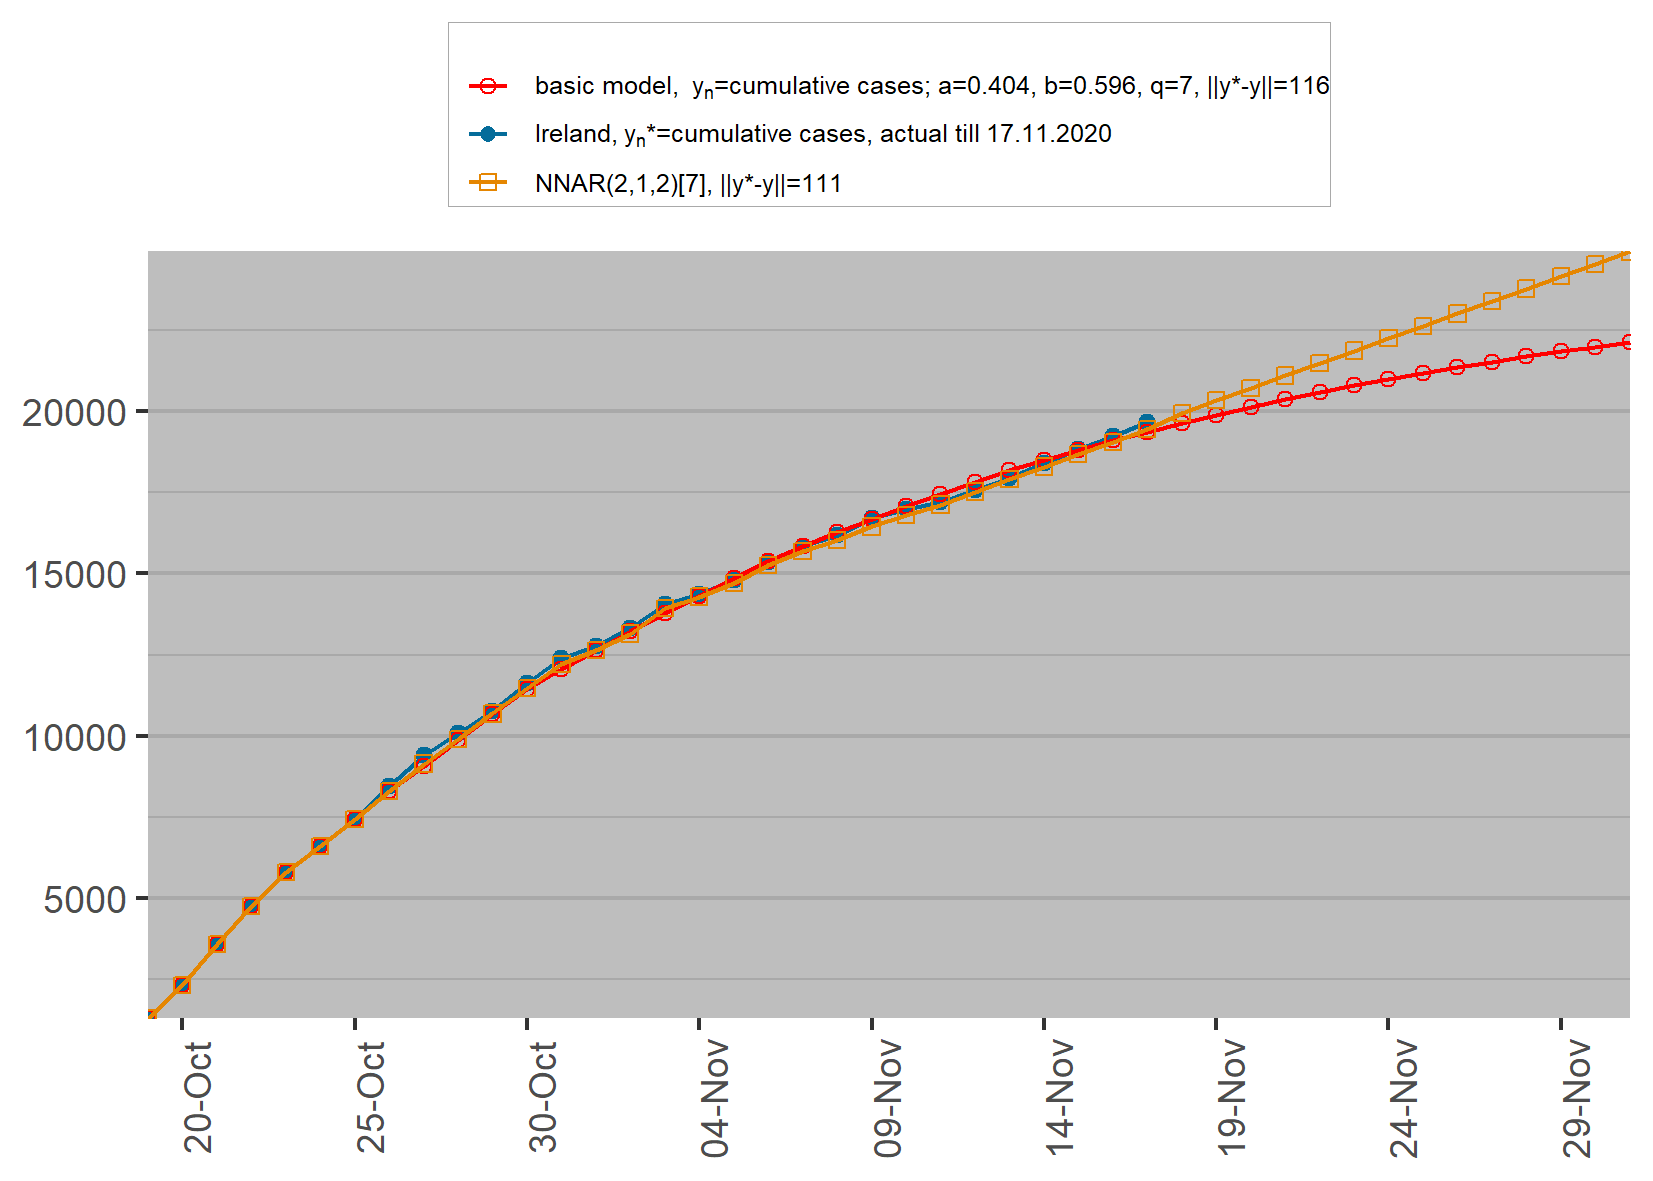
\includegraphics[width=\linewidth]{Ireland-nny.png} \label{fig:ireland-nny}
\endminipage
\caption{Neural Network model, Ireland}
\end{figure}
